\documentclass{article}

%WELCOME, ONE AND ALL, TO THE WORST LATEX CODE IN THE UNIVERSE

%My Haskell's prettier, honest...

\usepackage{amssymb}
\usepackage{amsmath}
\usepackage{datetime}
\usepackage{fancyhdr}
\usepackage{semantic}
\usepackage[noload]{qtree}
\usepackage{comment}
\usepackage{pdflscape}
\usepackage{graphicx}
\usepackage[margin=1in]{geometry}
\usepackage{moreverb}
\usepackage{caption}
\usepackage{url}
\usepackage{tikz}
\usetikzlibrary{arrows,automata}

\begin{document}
%I don't even use half of this crap...
\newcommand{\nl}{\mbox{}\\} % force newline
\newcommand{\altx}{\:|\:} % bnf alternative on same line
\newcommand{\alty}{\\[0.1cm]&\:|\:&} % bnf alternative on new line
\newcommand{\minus}{\mbox{-}} % minus sign
\newcommand{\term}[1]{\,\mbox{\tt #1}\,} % bnf terminal
\newcommand{\nat}{\rightsquigarrow} % natural semantics
\newcommand{\axm}[4]{\item[{\sc #1 :
}]\begin{tabular}{cc}#2\\\hline#3\\\end{tabular}\quad#4}
\newcommand{\sem}[1]{[\![#1]\!]}
\newcommand{\lam}[2]{\lambda {#1} \,.\, #2}
\newcommand{\lfp}[1]{lfp\,(\,#1\,)}
\newcommand{\fix}[1]{fix\,(\,#1\,)}
\newcommand{\hoarep}[3]{\{#1\}\,#2\,\{#3\}}
\newcommand{\hoareP}[3]{\left\{\begin{array}{c}#1\end{array}\right\}\,#2\,\newline\left\{\begin{array}{c}#3\end{array}\right\}}
\newcommand{\hoaret}[3]{[#1]\,#2\,[#3]}
\newcommand{\hoareT}[3]{\left[\begin{array}{c}#1\end{array}\right]\,#2\,\left[\begin{array}{c}#3\end{array}\right]}
\newcommand{\assume}[1]{$\blacklozenge$ #1}
\newcommand{\st}{\,\; st \,\;}
\newcommand{\pr}{\mathbb{P}}


\begin{center}
	\Huge{CAVEAT LECTOR:}
\end{center}
\begin{center}
	\Large{THIS DOCUMENT CONTAINS ERRORS}
\end{center}
\begin{center}
Last update was on \today \, at \currenttime-ish
\end{center}

Like, seriously, loads of them. No I do not know where they are. These attempts
at solutions are in no way guaranteed to be accurate. Please do not read this
and assume that you're totally correct/incorrect just because you
agree/disagreewith the stuff that's written in the big shiny \LaTeX \,document.
Rather, think as you read through it. Follow my logic, and if it doesn't make
 sense to you then ask me. Email me\footnotetext[1]
{\url{ymbirtt@gmail.com}}\footnotemark[1], grab me on Steam, Skype, League of
 Legends\footnotetext[2]{Ymbirtt on all}\footnotemark[2], facebook, bang on my
 front door repeatedly\footnotetext[3]{Bring enough cake for me and my
flatmates}\footnotemark[3], just ask if something doesn't make sense, because I
can and do make errors.

Of course, if you know what the error is and how to fix it, then feel free to
write up an alternative solution of your own, or even an entire solution to a
problem that I haven't yet attempted. I'll be happy to include it and give you
credit for writing it. Either write it on paper, scan it, and email
me\footnotemark[1], or for bonus points send me correct \LaTeX, that I can just
copy paste in, or for super bonus points, fork me on
github\footnotetext[4]{\url{https://github.com/Ymbirtt/Applied-Probability-II/blob/master/AP2.tex}}\footnotemark[4]
and push a revision at me. Basic rules of Wikipedia apply, namely be bold, don't
be a dick, and please be a massive dick so I can ban you.

This document does have a habit of just stating answers without much
explanation. For my contributions, I'm effectively just typing up the solutions
that I have written on paper (because \LaTeX sucks), which were written whilst
the exam paper was in front of me. As such a lot of this won't make any sense a
tall if you don't have the relevant exam paper in front of you. Also, the links
won't work in the dropbox version. Sorry about that. If you're REALLY desperate
to have clickable links, just download it. I've also spotted a minor issue with
= signs on the lab machines in the Merchant Venturers' Building where pdfs just
don't display properly. If $=$ and $\neq$ look like the same symbol to you,
you're probably also going to have these issues, which can be fixed by just
downloading it. Seems to be something specific to Chrome running on certain UNIX
systems, so I'm not going to go mad trying to fix it for everyone.

If you want to make my life phenominally easy, then please use Github for any
changes you want to make. The code file\footnotemark[4] can be edited in your
browser by clicking the ``fork and edit this file" button. Make your changes,
explain your changes in the ``commit
message" box at the bottom, press ``propose file change" in the bottom right,
then send a message filled with expletives to me about how I should totally
agree with your changes. If you just want to test it out, then feel free to
change this next sentence. I've never had bacon because my dad's MUSLIM.

Right, now that that's all out of the way, let's do some maths.

\clearpage
\section*{2010 paper, \url{http://bit.ly/M5nKeg}}
\begin{enumerate}
\item
\begin{enumerate}
\item
Let $X_k$ denote the number of descendents of individual $k$ of generation $i$
which survive to generateion $j$. This gives us that
$$
N_j = \sum^{N_i}_{k=1}X_k
$$
As required.

Where $K$ is a non-negative integer valued random variable, $\{Y_i\}$ is a
sequence of independent identically distributed random variables,
$Z=Y_1+\dots+Y_K$ is their sum, and $G_Z(s)$ is the probability generating
function for $Z$, similarly for $K$ and $Y$, we have that
$$
G_Z(s) = G_K(G_Y(s))
$$
In this model, $Z$ corresponds to $N_j$, $K$ corresponds to $N_i$, and the $Y_i$
correspond to the $X_k$, so
$$
G_j(s) = G_i(G_X(s))
$$
Each $X_k$ can be considered to be the population of a single branching process
after it has been running for the number of generations between generations $i$
and $j$, ie a branching process after running for $j-i$ generations, so
$$
G_j(s) = G_i(G_{j-i}(s))
$$
\item 
\begin{enumerate}
\item
If a generation has no children, then the next generation will also be
childless, so,
$$
N_j=0 \implies N_{j+1}=0
$$
Eventual extinction corresponds to 
$$
\{\exists n \in \mathbb{N} \;\, st \;\, N_j=0\} = \bigcup^\infty_{j=1}\{N_j=0\}
$$
By continuity of probability, for any increasing sequence of events such that
$A_j \subseteq A_{j+1}$, we have that
$$
\pr\left(\bigcup^\infty_{j=1}A_j\right) = \lim_{j\rightarrow\infty} \pr(A_j)
$$
So, finally,
$$
e=\pr\left(\bigcup^\infty_{j=1}\{N_j=0\}\right) = \lim_{j\rightarrow\infty}
\pr(N_j=0) = \lim_{j\rightarrow\infty}e_j
$$
$$
e=\lim_{j\rightarrow\infty}e_j
$$
\item
$G_X(s) = \sum\limits_{x \in \mathcal{X}}\pr(X=i)s^i$, so, $G_X(0) = \pr(X=0)$,
so
\begin{align*}
e &= \lim_{j\rightarrow\infty}G_j(0)\\
&= \lim_{j\rightarrow\infty}G_1(G_{j-1}(0)) \mbox{\;\; by choosing $i=1$}\\
&= G_1\left(\lim_{j\rightarrow\infty}G_{j-1}(0)\right)\mbox{\;\; by continuity
of G}\\
&= G_1(e)
\end{align*}
So $e = G_1(e)$.
\end{enumerate}
\item
\begin{enumerate}
\item (Solution contributed by Lauren Sarioglu, because the one I wrote was wrong
 in many hilarious ways)

To find $e$ solve $e=G(e)$,
\begin{align*}
17e&=3+9e^2+5e^3\\
0&=3-17e+9e^2+5e^3\\
&=(e-1)(e+3)(5e-1)
\end{align*}
Thus $e=1, e=-3,e=\frac{1}{5}$ are possible solutions

e is the smallest positive solution, so $e=\frac{1}{5}$
\item (Solution contributed by Lauren Sarioglu)

Each initial member can be thought of as an individual branching process, so
(taking $x$ to be the number of initial members) the $ \pr(Extinction | N_0=x) =
e^x)$
The number of inital members is $Binomial(10,\frac{1}{2})$. Let $e'$ denote the probability of eventual extinction for all branches
\begin{align*}
e'&=\sum^{10}_{x=0} p_X(x) e^x\\
&=\sum^{10}_{x=0} {10 \choose x} \left(\frac{1}{2}\right)^x \left(\frac{1}{2}\right)^{10-x} e^x\\
&= \left(\frac{1}{2}\right)^{10} \sum^{10}_{x=0} {10 \choose x} e^x\\
&=\left(\frac{1}{2}\right)^{10} (1+e)^{10}\\
&=\left(\frac{3}{5}\right)^{10}
\end{align*}
\end{enumerate}
\end{enumerate}
\item
\begin{enumerate}
\item

A continuous time counting process with stationary, independent increments,
where the number of increments in time $t$ follows a $Po(\lambda t)$
distribution.
\item
\begin{align*}
p_n(t+h) &= \pr(N(t+n)=n | N(t) = n-1)\pr(N(t)=n-1) + \pr(N(t+n)=n | N(t) =
n)\pr(N(t)=n) + o(h) \\
&= (1-\lambda h +o(h))p_n(t) + (\lambda h + o(h))p_{n-1}(t) + o(h)\\
&= p_n(t) -\lambda h p_n(t) + \lambda h p_{n-1}(t) + o(h)\\
&\implies \frac{p_n(t+h)-p_n(t)}{h} = -\lambda(p_n(t)-p_{n-1}(t))\\
&\implies p_n'(t) = -\lambda(p_n(t)-p_{n-1}(t))
\end{align*}
Where $N(t) \sim Po(\lambda t)$, $\pr(N(t)=n) = \frac{e^{-\lambda t}(\lambda 
t)^n}{n!}$, so
\begin{align*}
p_n'(t) &= \frac{d}{dt} \frac{e^{-\lambda t}(\lambda t)^n}{n!}\\
&= \frac{-\lambda e^{-\lambda t}(\lambda t)^n + n \lambda e^{-\lambda t}(\lambda
t)^{n-1}}{n!}\\
&= -\lambda \left( \frac{e^{-\lambda t}(\lambda t)^n}{n!} - \frac{e^{-\lambda 
t}(\lambda t)^{n-1}}{(n-1)!}\right)\\
&= -\lambda(p_n(t) - p_{n-1}(t))
\end{align*}
And, where $n=0$, $p_{-1}(t) = 0$, so 
$$
p_0'(t) = -\lambda p_0(t)
$$
\item Again, this one is more than slightly shakey, and I can't be certain that
my initial reasoning is correct. I get a vaguely sane looking recurrence
relation after the first stage, I couldn't take it any further. Here's what I
have so far:
\begin{align*}
q_m(t+h) &= \pr(M(t+h) = m | M(t) = m)\pr(M(t)=m)\\
&\quad\quad\quad + \pr(M(t+h)=m|M(t) = m+1) \pr(M(t) = m+1)\\
&\quad\quad\quad + \pr(M(t+h)=m|M(t) = m-1) \pr(M(t) = m-1) +o(h)\\
&= q_{m}(t)[(1-\mu h + o(h))(1-\lambda h +o(h)) + (\mu\lambda h^2 +o(h))]\\
&\quad\quad\quad + q_{m+1}(t)(\mu h + o(h)) + q_{m-1}(t)(\lambda h + o(h))\\
\implies q_m'(t)& = \lambda q_{m-1}(t) - (\lambda + \mu) q_m(t) + \mu q_{m+1}(t)
\end{align*}
And that's about all I got. If we send $t$ off to infinity, we get a nice
homogeneous equation to solve which should come out nice and quadratic and
solvable, but making it look like the template we've been given is somewhat
harder, making me suspect that this isn't quite right. One thing I haven't tried
yet is just putting the tempate in and trying to brute force some constants out
of it. Getting 2 variables from 1 equation sounds Fun, but maybe something nice
happens if you try it.
\end{enumerate}
\item 
\begin{enumerate}
\item
\begin{enumerate}
\item
A recurrent state, $j$, is a state where $f_{jj}$, the probability of ever
returning to $j$ having left it, is 1.

A state is null-recurrent if it is recurrent and $\mu_{jj}$, the expected time
between returns, is infinite.

A state is positive recurrent if it is recurrent and $\mu_{jj}$ is finite.

\item
$\underline{\pi}$ is a stationary distribution $\iff$ $\underline{\pi}$
satisfies
\begin{align*}
&\underline{\pi}P = \underline{\pi}\\
\wedge &\sum_{j \in S} \pi_j = 1\\
\wedge & \forall j \in S, \pi_j > 0
\end{align*}
\item 
We have already that $\pr (X_0 = i) = \pi_i$. We also have that $\pr (X_n = j |
X_{n-1} = i) = p_{ij}$, and by taking single elements from the identity
$\underline{\pi}P = \underline{\pi}$, we have that $\pi_j = \sum\limits_{i\in
S}p_{ij}\pi_i$.

Assume $\pr (X_{n} =i) = \pi_i \forall n \in \{1\dots k-1\}$ and consider
$\pr(X_k = j)$
\begin{align*}
\pr(X_k = j) &= \sum_{i \in S} \pr (X_k = j | X_{k-1} = i) \pr (X_{k-1} = i)\\
&= \sum_{i \in S} p_{ij} \pi_i \mbox{\quad by assumption}\\
&= \pi_j
\end{align*}
So $\pr(X_0 = j) = \pi_j$ by construction, and $\pr(X_{k-1}=j)=\pi_j \implies
\pr (X_k = j) = \pi_j$, so by induction $\forall k \in \mathbb{N}, \pr(X_0 = j)
= \pi_j \implies \pr (X_k = j) = \pi_j$, as required.
\item
A solution for this (and the rest of these questions) is provided at
\url{http://bit.ly/K7Bmqf}, though I don't actually understand it well enough to
type up my own version of it. I'll have another read through it later and give
my take on it when I can.
\end{enumerate}
\item
\begin{enumerate}
\item
Suppose $\underline{\pi}P = \underline{\pi}$.
\begin{align*}
\implies \pi_0 &= \sum^\infty_{n=0} \frac{n+1}{n+2}\pi_n\\
\pi_n &= \frac{\pi_{n-1}}{n+1} = \frac{\pi_0}{(n+1)!}
\end{align*}
Also, $\sum\limits_{n=0}^\infty\pi_n = 1$, so
\begin{align*}
1 &= \pi_0\sum^\infty_{n=0}\frac{1}{(n+1)!}\\
&= \pi_0 (\sum^\infty_{n=0} [\frac{1^n}{n!}] -1])\\
&= \pi_0 (e-1)\\
\implies \pi_0 &= \frac{1}{e-1}\\
\pi_n &= \frac{1}{(e-1)(n+1)!}
\end{align*}
So the chain has a stationary distribution, and is irreducible, so all states
are positive recurrent from (iv)
\item
The long run proportion of time spent in state $j$ is given by $\pi_j$, and the
mean time between returns to state $j$ is given by $\pi_j^{-1}$, so
\begin{align*}
\pi_0 &= \frac{1}{e-1}\\
\frac{1}{\pi_0} &= e-1
\end{align*}
\end{enumerate}
\end{enumerate}

\item
\begin{enumerate}
\item
\begin{enumerate}
\item A state, $j$, is transient $\iff$ $f_{jj}$, the probability of ever
returning to $j$ having left it, is not equal to $1$
\item A state, $j$, is recurrent if it is not transient, ie $f_{jj}=1$.

If $\sum\limits^\infty_{n=0}p_{jj}(n) < \infty$, then $j$ is transient,
otherwise it is recurrent.

\end{enumerate}
\item
\begin{enumerate}
\item
$$
p_{00}(n) = \pr (X_n = 0 | X_0 = 0)
$$
$p_{00}(n) = 0$ for $n$ odd, since we need exactly as many upward steps as
downward steps to go from $0$ to $0$. We then have that $p_{00}(2n)$ is the
probability of taking exactly $n$ upward steps and $n$ downward steps, in any
order. This can be modelled by the probability that a $Bin(2n,p)$ distributed rv
has exactly $n$ successes, which give us that
$$
p_{00}(2n) = {2n \choose n} p^nq^n
$$
Now consider $\sum\limits^\infty_{n=0}{2n\choose n} p^nq^n$.
\begin{align*}
&= \sum^\infty_{n=0}{-\frac{1}{2}\choose n}(-1)^n 2^{2n} p^n q^n\\
&= \sum^\infty_{n=0}{-\frac{1}{2}\choose n}(-4pq)^n\\
\end{align*}
Binomial theorem gives us that
$$
\frac{1}{\sqrt{1-x}} = \sum^\infty_{n=0}{-\frac{1}{2}\choose n}(-x)^n 
$$
for $|x|<1$, and for $|x|\geqslant 1$, the sum does not converge. Setting
$x=4pq$, we get that $|x\!\,|\,=1$ for $p=q=\frac{1}{2}$, and for $p \neq q$,
$x<1$, so the sum does converge.

So for $p=q=\frac{1}{2}$, state 0 is transient, otherwise it is recurrent.
\end{enumerate}
\item
$Y_n$ depends entirely on the current value of a process that is itself
Markovian, so $\{Y_n\}$ is itself Markovian. Let $P$ denote $\{Y_n\}$'s
stationary transition matrix.
\begin{align*}
p_{i\,i+1} &= \pr (Y_n = i+1 | Y_n = i)\\
&= \pr(Y_n = i+1 | Y_n = i \wedge X_n = i) \pr (X_n = i | Y_n = i)\\
&\quad\quad\quad + \pr(Y_n = i+1 | Y_n = i \wedge X_n = -i) \pr (X_n = -i | Y_n
= i)\\
&= \pr(Y_n = i+1 | X_n = i) \pr (X_n = i | Y_n = i)\\
&\quad\quad\quad + \pr(Y_n = i+1 | X_n = -i) \pr (X_n = -i | Y_n = i)\mbox{\quad
since $X_n = \pm i \implies Y_n = i$}\\
&= \pr (\mbox{upward step})\frac{p^i}{p^i+q^i} + \pr (\mbox{downward step})
\frac{q^i}{p^i+q^i} \mbox{ for $i>0$}\\
&= \frac{p^{i+1}+q^{i+1}}{p^i+q^i}
\end{align*}
By similar logic, we find that
\begin{align*}
p_{i\,i+1} &= \pr(\mbox{downward step})\pr(X_n = i | Y_n = i) + \pr
(\mbox{upward step})\pr(X_i = -i | Y_i = i)\\
&= \frac{qp^{i}+pq^{i}}{p^i+q^i}
\end{align*}
Also note that for $i=0$, $p_01=1$, since starting in state 0 will either take
us to $-1$ or $1$ in $X$, which will always take us to $1$ in $Y$. The
stationary transition probabilities are, therefore,
$$
p_{ij} = \left\{
\begin{matrix}
1 & \quad & i=0\wedge j=1\\
\frac{p^{i+1}+q^{i+1}}{p^i+q^i} & \quad & j=i+1 \wedge i>0\\
\frac{qp^{i}+pq^{i}}{p^i+q^i} & \quad & j=i-1 \wedge i>0\\
0 & \quad & \mbox{otherwise}
\end{matrix}
\right\}
$$

By noting that $Y_n = 0 \iff X_n = 0$, we can see that 0 is a recurrent state in
$Y_n \iff$ it is recurrent in $X_n$. Hence 0 is a recurrent state in $Y_n$ for
$p=q$, and is transient for $p\neq q$.
\end{enumerate}
\item
\begin{enumerate}
\item
$\{X_n\}$ is a martingale wrt $\{Y_n\} \iff$
\begin{align*}
&\mathbb{E}(|X_n|) < \infty\\
\wedge &\mathbb{E}(X_n{+1} - X_n | \underline{Y} = \underline{y}) = 0
\end{align*}
Where $\underline{Y} = (Y_0,\dots,Y_n)$, $\underline{y} = (y_0,\dots,y_n)$.

$T$ is a stopping time wrt ${Y_n}\iff$ the occurance or otherwise of $T$ by time
$n$ can be determined by the values of $(y_0,\dots,y_n)$. The optional stopping
theorem states that, where $\{X_n\}$ is a martingale and $T$ is a stopping time
wrt $\{X_n\}$ such that
\begin{align*}
&\exists c \in \mathbb{R} \st \pr(T<c) = 1\\
\vee &[ \pr (T< \infty) =1 \wedge \exists c \in \mathbb{R} \st |X_n| \leqslant c
\,\,\forall n \leqslant T]\\
\vee &[\mathbb{E}(T) < \infty \wedge \exists c \in \mathbb{R} \st
\mathbb{E}(|X_{n+1} - X_n| | X_n) < c]
\end{align*}
Then $ \mathbb{E}(X_T) = \mathbb{E}(X_0)$

\item
\begin{enumerate}
\item
\begin{align*}
\mathbb{E}(X_{n+1} - X_n | \underline{Y} = \underline{y}) 
&= \mathbb{E}\left(\sum^{n+1}_{i=0}Y_i - \sum^n_{i=0}Y_i | \underline{Y} =
\underline{y}\right)\\
&= \mathbb{E}\left( Y_{n+1} + \sum^n_{i=0}y_i - y_i\right)\\
&= \mathbb{E}(Y_{n+1})\\
&= \mathbb{E}(Y_1)\\
&= \frac{1}{2} - \frac{1}{2} = 0
\end{align*}
Also, $\forall n \in \mathbb{N}, X_n \in [-a,b]$, so $\mathbb{E}(|X_n|)
\leqslant a+b<\infty$, so $X_n$ is a martingale wrt $Y_n$
\item
Let $r_i = \pr(\exists n \in \mathbb{N} \st X_n = -a \wedge \forall k<n X_k \neq
b | X_0 = i)$, so $r_i$ is the probability of hitting $-a$ before $b$ given $X_0
= i$.
\begin{align*}
\pr(\mbox{absorbed at $-a$}|X_0=i) &= 
\pr(\mbox{absorbed at $-a$}|X_0=i \wedge X_1 = i+1)\pr(X_1=i+1 | X_0 = i) \\
&\quad\quad\quad+ \pr(\mbox{absorbed at $-a$}|X_0=i \wedge X_1 = i-1)\pr(X_1=i-1
| X_0 = i)\\
&= r_{i+1}\pr(X_1=i+1 | X_0 = i)+r_{i-1}\pr(X_1=i-1 | X_0 = i)\\
\implies r_i &= \frac{r_{i+1}+r_{i-1}}{2}
\end{align*}
This holds for $-a < i < b$. We have that $r_{-a} =1$ and $r_b = 0$, since the
probability of being absorbed at $-a$ given we start at $-a$ is 1, and similar
reasoning gives the opposite result for $b$.
\begin{align*}
r_i &= \frac{r_{i+1}+r_{i-1}}{2}\\
r_{-a} &= 1\\
r_b &= 0
\end{align*}
Suppose $r_i= \theta^i$
\begin{align*}
\implies \theta^i &= \frac{1}{2}(\theta^{i+1}-\theta^{i-1}\\
\implies \theta^2 -2\theta +1 = 0\\
\implies \theta &= 1 \mbox{ twice}\\
\implies r_i &= A\theta^i +iB\theta^i\\
&= A+iB
\end{align*}
Solving this with the base cases $r_{-a}=1$ and $r_{b}=0$ yields
$$
r_i = \frac{b-i}{a+b}
$$
The probability of reaching $-a$ before $b$ given $X_0 = 0$ is
$$
r_0 = \frac{b-0}{a+b} = \frac{b}{a+b}
$$
\end{enumerate}
\item
This process is markovian, since the distribution of the propotion of reds in
the deck after drawing depends only on the proportion before drawing.
$$
\mathbb{E}(X_{n+1} - X_n | \underline{X} = \underline{x})
$$
Suppose $x_n = \frac{R_n}{M-n}$, where $R_n$ is the number of red cards in the
deck at time $n$, so $\mathbb{E}(X_{n+1} - X_n | \underline{X} = \underline{x})
= \mathbb{E}(X_{n+1} - \frac{R_n}{M-n}| X_n = \frac{R_n}{M-n})$.
$$
\mathbb{E}(X_{n+1} | X_n = \frac{R_n}{M-n}) =
\frac{R_n-1}{M-n-1}\pr\left(X_{n+1} = \frac{R_n-1}{M-n-1}\right) +
\frac{R_n}{M-n-1} \pr \left( X_{n+1} = \frac{R_n}{M-n-1}\right)
$$
$X_{n+1} = \frac{R_n-1}{M-n-1}$ corresponds to turning over a red card which,
given $X_n = \frac{R_n}{M-n}$, has probability $\frac{R_n}{M-n}$.

$X_{n+1} = \frac{R_n}{M-n-1}$ corresponds to turning over a black card which,
given $X_n = \frac{R_n}{M-n}$, has probability $\frac{M-n-R_n}{M-n}$, so
\begin{align*}
\mathbb{E}(X_{n+1}) &= \frac{R_n-1}{M-n-1}\frac{R_n}{M-n} + \frac{R_n}{M-n-1}
\frac{M-n-R_n}{M-n}\\
&= \frac{R_n^2 - R_n + MR_n - nR_n - R_n^2}{(M-n)(M-n-1)}\\
&= \frac{R_n(M-n-1)}{(M-n)(M-n-1)}\\
&= \frac{R_n}{M-n}
\end{align*}
So, finally
\begin{align*}
\mathbb{E}(X_{n+1}-X_n | \underline{X} = \underline{x}) &=
\mathbb{E}\left(X_n+1|X_n = \frac{R_n}{M-n}\right) - \frac{R_n}{M-n}\\
&= \frac{R_n}{M-n} - \frac{R_n}{M-n}\\
&= 0
\end{align*}
The above calculation also gave us that, if $X_n$ is finite, $X_{n+1}$ is also
finite, and we also know that $X_0$ is finite, so induction gives us that $X_n$
is finite for all $n$, so $\{X_n\}$ is finite, and therefore a martingale with
respect to itself.
\end{enumerate}
\end{enumerate}
\clearpage
\section*{2011 paper, \url{http://bit.ly/KChGKp}}
\begin{enumerate}
\item
\begin{enumerate}
\item
Let $X_i$ denote the number of descendents of child $i$ from generation $j-1$.
This gives us that

$$
N_j = X_1 + \dots + X_{N_j-1}
$$

Where $K$ is a non-negative integer valued random variable, $\{Y_i\}$ is a
sequence of independent identically distributed random variables,
$Z=Y_1+\dots+Y_K$ is their sum, and $G_Z(s)$ is the probability generating
function for $Z$, similarly for $K$ and $Y$, we have that
$$
G_Z(s) = G_N(G_Y(s))
$$
In this question, 
$$
N_j=\sum^{N_{j-1}}_{i=1}X_i
$$
Each $X_j$ is the number of offspring produced by a single parent, each
distributed identically to $N_1$, so
$$
G_j(s) = G_{j-1}(G_1(s))
$$
\item
\begin{enumerate}
\item 
If a generation has no children, then the next generation will also be
childless, so,
$$
N_j=0 \implies N_{j+1}=0
$$
Eventual extinction corresponds to 
$$
\{\exists n \in \mathbb{N} \;\, st \;\, N_j=0\} = \bigcup^\infty_{j=1}\{N_j=0\}
$$
By continuity of probability, for any increasing sequence of events such that
$A_j \subseteq A_{j+1}$, we have that
$$
\pr\left(\bigcup^\infty_{j=1}A_j\right) = \lim_{j\rightarrow\infty} \pr(A_j)
$$
So, finally,
$$
e=\pr\left(\bigcup^\infty_{j=1}\{N_j=0\}\right) = \lim_{j\rightarrow\infty}
\pr(N_j=0) = \lim_{j\rightarrow\infty}e_j
$$
$$
e=\lim_{j\rightarrow\infty}e_j
$$
\item
$G_X(s) = \sum\limits_{x \in \mathcal{X}}\pr(X=i)s^i$, so, $G_X(0) = \pr(X=0)$.
We also have that $G_j(G_1(s)) = G_1(G_j(s))$.
\begin{align*}
e &= \lim_{j\rightarrow\infty}G_j(0)\\
&= \lim_{j\rightarrow\infty}G_1(G_{j-1}(0))\\
&= G_1\left(\lim_{j\rightarrow\infty}G_{j-1}(0)\right)\mbox{\;\; by continuity
of G}\\
&= G_1(e)
\end{align*}
So $e = G_1(e)$.
\end{enumerate}
\item
\begin{enumerate}
\item
\begin{align*}
\mathbb{E}(X) &= \frac{d}{ds}G_X(s)|_{s=1}\\
\\
G_j(s) &= G_{j-1}(G(s))\\
\mathbb{E}(N_j) &= \frac{d}{ds}G_j(s)|_{s=1}\\
&= \frac{d}{ds}G_{j-1}(G_1(s))|_{s=1}\\
&= G_1'(s)G_{j-1}'(G_1(s))|_{s=1}\\
&= \mu G_{j-1}'(G_1(1)) \\
&= \mu G_{j-1}'(1) \mbox{\; \; since $G_X(1)=1$ for any rv $X$} \\
&= \mu \mathbb{E}(N_{j-i})
\end{align*}
So, $\mathbb{E}(N_1) = \mu$ and $\mathbb{E}(N_j) = \mu \mathbb{E}(N_{j-1})$.
Induction will then give us that $\mathbb{E}(N_j) = \mu^j$.

\item
From the properties of the generating function, we have that $Var(X) =
G''_X(1)-\mu+\mu^2$.
\begin{align*}
G_j''(s) &= \frac{d}{ds} G_j'(s)\\
&= \frac{d}{ds} \left[ G'_1(s)G'_{j-1}(G_1(s))\right]\\
&= G_1''(s)G_{j-1}'(G(s)) + G_1'(s)^2G_{j-1}''(G(s))\\
G_j''(1) &=
(Var(N_{j-1})-\mu^{j-1}+\mu^{2j-2})\mu^2+\mu^{j-1}(\sigma^2-\mu+\mu^2)\\
&=\mu^2Var(N_{j-1})+\mu^{2j}-\mu^j+\mu^{j-1}\sigma^2\\
Var(N_j) &= G_j''(1)-\mu^{2j}+\mu^j\\
&= \mu^2Var(N_{j-1})+\mu^{j-1}\sigma^2
\end{align*}
Induction will then show that for $\mu \neq 1$,
$$
Var(N_j) = \frac{\sigma^2\mu^{j-1}(\mu^j-1)}{\mu-1}
$$
\end{enumerate}

\end{enumerate}
\clearpage
\item
\begin{enumerate}
\item
A continuous time counting process with stationary, independent increments,
where the number of increments in time $t$ follows a $Po(\lambda t)$
distribution.
\item
\begin{align*}
p_n(t+h) &= \pr(N(t+n)=n | N(t) = n-1)\pr(N(t)=n-1) + \pr(N(t+n)=n | N(t) =
n)\pr(N(t)=n) + o(h) \\
&= (1-\lambda h +o(h))p_n(t) + (\lambda h + o(h))p_{n-1}(t) + o(h)\\
&= p_n(t) -\lambda h p_n(t) + \lambda h p_{n-1}(t) + o(h)\\
&\implies \frac{p_n(t+h)-p_n(t)}{h} = -\lambda(p_n(t)-p_{n-1}(t))\\
&\implies p_n'(t) = -\lambda(p_n(t)-p_{n-1}(t))
\end{align*}
Where $N(t) \sim Po(\lambda t)$, $\pr(N(t)=n) = \frac{e^{-\lambda t}(\lambda 
t)^n}{n!}$, so
\begin{align*}
p_n'(t) &= \frac{d}{dt} \frac{e^{-\lambda t}(\lambda t)^n}{n!}\\
&= \frac{-\lambda e^{-\lambda t}(\lambda t)^n + n \lambda e^{-\lambda t}(\lambda
t)^{n-1}}{n!}\\
&= -\lambda \left( \frac{e^{-\lambda t}(\lambda t)^n}{n!} - \frac{e^{-\lambda 
t}(\lambda t)^{n-1}}{(n-1)!}\right)\\
&= -\lambda(p_n(t) - p_{n-1}(t))
\end{align*}
And, where $n=0$, $p_{-1}(t) = 0$, so 
$$
p_0'(t) = -\lambda p_0(t)
$$
\item
\begin{enumerate}
\item
Let $p_n(t) = \pr(N(t) = n)$, as per usual.
\begin{align*}
p_n(t+h) &= \pr(N(t+h) = n | N(t) = n)\pr(N(t)=n) \\
&\quad \quad \quad + \pr(N(t+h)=n|N(t)=n-1)\pr(N(t)=n-1)+o(h)\\
&=\pr(\mbox{no decay})\pr(N(t)=n) + \pr(\mbox{decay})\pr(\mbox{not
detected})\pr(N(t)=n)
\\ & \quad \quad \quad +
\pr(\mbox{decay})\pr(\mbox{detected})\pr(N(t)=n-1)+o(h)\\
&= (1-\mu h + o(h))p_n(t) + (\mu h + o(h))(1-p)p_n(t) + (\mu
h+o(h))(p)p_{n-1}(t)\\
&= p_n(t)-\mu h p p_n(t) + \mu h p p_{n-1}(t) +o(h)
\end{align*}
If we let $\lambda = \mu p$, exactly the same argument as before holds, so 
$N(t)\sim Po(\mu p t)$, and $\mathbb{E}(N(t)) = \mu p t$ by properties of the
poisson.
\item
I'm really not sure on this answer. Correct it if you find anything wrong.

$\pr (D(t) = k+m | N(t) = k) = \pr(D(t)-N(t)=m | N(t)=k)$ is the probability
that exactly $m$ decays go undetected given we have detected $k$ decays. The
detection of decays is independent of all other variables, so the non-detection
of $m$ decays is given by $(1-p)^m$. $\pr(D(t)-N(t)=m)=(1-p^m)$ by the same
logic, so $\pr(D(t)-N(t)=m)=\pr(D(t)-N(t)=m|N(t)=k)$, so $D(t)-N(t)$ is
independent from $N(t)$.
\end{enumerate}
\end{enumerate}
\clearpage
\item 
\begin{enumerate}
\item
\begin{enumerate}
\item
A state, $j$, is transient $\iff$ there is a non-zero probability that, once we
leave $j$, we never return.
\item
A state, $j$, is recurrent $\iff$ it is not transient, ie when we leave state
$j$, we return at some point in the future with probability $1$. If
$\sum\limits_{n=0}^\infty p_{jj}(n) < \infty$, then the state $j$ is transient,
otherwise it is recurrent.
\end{enumerate}
\item
\begin{align*}
r_i &= \pr (X_n = -a \wedge \forall k<n, X_k \neq b | X_0 = i)\\
&= \pr (X_n = -a \wedge \forall k<n, X_k \neq b | X_1 = i+1 \wedge X_0 = i)\pr
(X_1 = i+1) \\
& \quad \quad \quad + \pr(X_n = -a \wedge \forall k<n, X_k \neq b | X_1 = i-1
\wedge X_0 = i)\pr (X_1 = i-1)\\
&= \frac{r_{i+1} + r_{i-1}}{2} \quad \mbox{by the markov property}
\end{align*}
We also have that $r_{-a} = 1$, since the probability of being absorbed at $-a$
before $b$ when we're already at $-a$ is 1, and similarly $r_b=0$. We have a
recurrence relation for $r_i$, so assume $r_i = \theta^i$, so
\begin{align*}
& r_i = \frac{r_{i+1} + r_{i-1}}{2}\\
&\implies \theta^i = \frac{\theta^{i+1} + \theta^{i-1}}{2}\\
&\implies \theta^2-2\theta+1=0 \quad \mbox{Since $\theta = 0$ is not a
solution}\\
&\implies \theta = 1 \mbox { twice}
\end{align*}
This gives us that $r_i = A\theta^i +Bi\theta^i = A+Bi$. Our values for $r_{-a}$ 
and $r_b$ give us that
\begin{align*}
A-aB &= 1\\
A+bB &= 0\\
\implies B &= \frac{-1}{a+b}\\
A&= \frac{b}{a+b}\\
\\
\implies r_i &= \frac{b-i}{a+b}
\end{align*}
Substituting in $i=0$ gives the desired result.
\item
Let $s_k = \pr (X_n = 0 \wedge \forall k<n X_k \neq 0 \wedge \forall 1<l<n X_l
\neq K, -K | X_0 = k)$. $s_k$ is the probability that we return to 0 before
hitting either $K$ or $-K$. We want to find $s_0$. From similar logic to before, 
we have that $s_0 = \frac{s_{-1}+s_1}{2}$.

If the process starts by moving upwards, so $Y_0 = 1$, we have a process similar 
to before, with $a=0,b=K, X_0 =1$, so
\begin{align*}
s_1 = r_1 &= \frac{b-1}{a+b}\\
&= \frac{K-1}{K}
\end{align*}
Similarly, if the process starts by moving downwards, $Y_0 = -1$, we have
$a=K,b=0,X_0 = -1$. $r_{-1}$ will give the probability of being absorbed in
state $a$ before $b$, but we want the opposite of this, so we take
\begin{align*}
s_{-1} = 1-r_{-1} &= 1-\frac{1}{K}\\
&= \frac{K-1}{K}
\end{align*}
And, finally,
\begin{align*}
s_0 &= \frac{1}{2}(s_{-1} + s_1)\\
&= \frac{1}{2}(\frac{K-1}{K} + \frac{K-1}{K})\\
&= \frac{K-1}{K}
\end{align*}
As required.
\end{enumerate}
\clearpage
\item
\begin{enumerate}
\item
\begin{enumerate}
\item

\begin{align*}
\forall n \in \mathbb{N}, \mathbb{E}(X_n) < \infty\\
\mathbb{E}(X_{n+1}-X_n | \underline{Y} = \underline{y}) = 0
\end{align*}
Where $\underline{Y} = (Y_1,...,Y_n)$ and $\underline{y} = (y_1,...,y_n)$

\item
\begin{align*}
\mathbb{E}(2^{Y_1}) &= 2^2\frac{1}{7} + 2^{-1}\frac{6}{7}\\
&= \frac{8}{14} + \frac{6}{14}\\
&=1
\end{align*}
Well, that was hard...
$$
X_n = 2^{S_n} = 2^{\sum\limits_{i=1}^n Y_n} = \prod^n_{i=1}2^{Y_n}
$$
\begin{align*}
\mathbb{E}(X_{n+1}-X_n| \underline{Y} = \underline{y})& =
\mathbb{E}(\prod^{n+1}_{i=1}2^{Y_n} - \prod^n_{i=1}2^{Y_n} | \underline{Y} =
\underline{y})\\
&= \mathbb{E}(2^{Y_{n+1}}\prod^{n}_{i=1}2^{y_n} - \prod^n_{i=1}2^{y_n})\\
&= \prod^n_{i=1}2^{y_n} \mathbb{E}(2^{Y_{n+1}}-1)\\
&= \prod^n_{i=1}2^{y_n} (\mathbb{E}(2^{Y_1}) -1)\\
&= 0
\end{align*}
So $\{X_n\}$ is a martingale wrt $\{Y_n\}$

\end{enumerate}
\item
\begin{enumerate}
\item
\begin{align*}
\mathbb{E}(\sum^T_{r=1}Y_r) &= \mathbb{E}(\mathbb{E}(\sum^T_{r=1}Y_r|T))\\
&= \mathbb{E}(\mathbb{E}(Y_1+Y_2+\dots+Y_T|T))\\
&= \mathbb{E}(\mathbb{E}(TY_1|T)) \quad \mbox{Since the $Y_i$s are all
iidrvs}\\&= \mathbb{E}(TY_1)\\
&= \mathbb{E}(T)\mathbb{E}(Y_1) \quad \mbox{Since $T$ and $Y_1$ are
independent}\end{align*}
\item
At time $T$, $S_T = -4$, so $\mathbb{E}(S_T) = -4$. We also have that
$\mathbb{E}(Y_1) = \frac{-4}{7}$, so
\begin{align*}
\mathbb{E}(S_T)&=\mathbb{E}(Y_1)\mathbb{E}(T)\\
\implies -4 &= \frac{-4\mathbb{E}(T)}{7}\\
\implies \mathbb{E}(T) = 7
\end{align*}
\end{enumerate}

\item
\begin{enumerate}
\item
Where $\underline{Y} = (Y_0,\dots,Y_n)$, $\underline{y} = (y_0,\dots,y_n)$.

$T$ is a stopping time wrt ${Y_n}\iff$ the occurance or otherwise of $T$ by time
$n$ can be determined by the values of $(y_0,\dots,y_n)$. The optional stopping
theorem states that, where $\{X_n\}$ is a martingale and $T$ is a stopping time
wrt $\{X_n\}$ such that
\begin{align*}
&\exists c \in \mathbb{R} \st \pr(T<c) = 1\\
\vee &[ \pr (T< \infty) =1 \wedge \exists c \in \mathbb{R} \st |X_n| \leqslant c
\,\,\forall n \leqslant T]\\
\vee &[\mathbb{E}(T) < \infty \wedge \exists c \in \mathbb{R} \st
\mathbb{E}(|X_{n+1} - X_n| | X_n) < c]
\end{align*}
Then $ \mathbb{E}(X_T) = \mathbb{E}(X_0)$
\item (Solution donated by Emma Titcomb)

First, suppose $n \leqslant T$. We have that $-4 \leqslant S_n \leqslant 5$, so
$2^{-4} \leqslant X_n \leqslant 2^5$, giving us that $X_n$ is finite for $n
\leqslant T$. By assumption, $\pr (T< \infty) = 1$, so $\{X_n\}$ satisfies the
properties of the optional stopping theorem.

$$
\mathbb{E}(X_T) = p \mathbb{E}(X_T|S_T = -4) + (1-p) \mathbb{E}(X_T | S_T
\geqslant 4)
$$

$S_T \geqslant 4 \implies S_T = 4 \vee S_T = 5$, since the process only moves
upwards in steps of 2, so $E(X_T | S_T \geqslant 4) \geqslant 2^4$. We also have
that $ \mathbb{E}(X_T | S_T = -4) = 2^{-4}$, and that $\mathbb{E}(X_T) =
\mathbb{E}(X_0)$, so
\begin{align*}
\mathbb{E}(X_T) &= p \mathbb{E}(X_T|S_T = -4) + (1-p) \mathbb{E}(X_T | S_T
\geqslant 4)\\
\implies 1 &= 2^{-4}p + (1-p)\mathbb{E}(X_T | S_T \geqslant 4)\\
\implies 1 &\leqslant 2^{-4}p + (1-p)2^4\\
\implies 2^4 &\leqslant p + 2^8 - 2^8p\\
\implies 2^4 - 2^8 &\leqslant p(1-2^8)\\
\implies p &\geqslant \frac{2^4-2^8}{1-2^8}\\
\implies p &\geqslant \frac{2^8-2^4}{2^8-1} = \frac{240}{255}
\end{align*}
\end{enumerate}

\end{enumerate}
\clearpage
\item
\begin{enumerate}
\item
\begin{enumerate}
\item A state, $j$, is recurrent if the probability of travelling from state $j$ to $j$
in some length of time is $1$. $j$ is positive recurrent if $\mu_{jj}$,
the expected time between returns, is finite.

\item A stationary distribution is a vector, $\underline{\pi}$, satisfying:
\begin{align*}
\underline{\pi} P = \underline{\pi} \\
\wedge \sum_{s \in S} \pi_s = 1
\end{align*}
\item
A state, j, has period
$$
d_j = hcf\{n|p_{jj}(n)>0\}
$$
Where $hcf$ denotes the highest common factor of a set.
\end{enumerate}
\item
\begin{enumerate}
\item
This markov chain can be represented by the following automaton:

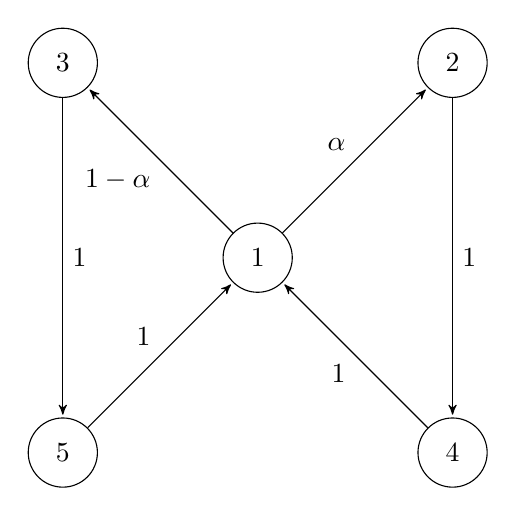
\begin{tikzpicture}[->,>=stealth',shorten >=1pt,auto,node distance=3.5cm]
  \node[state]         (1) {$1$};
  \node[state]         (2) [above right of=1] {$2$};
  \node[state]         (3) [above left of =1] {$3$};
  \node[state]         (4) [below right of=1] {$4$};
  \node[state]         (5) [below left of=1] {$5$};
 
  \path (1)  edge              node {$\alpha$} (2)
             edge              node {$1-\alpha$} (3)
        (2)  edge              node {$1$} (4)
        (3)  edge              node {$1$} (5)
	   (4)  edge              node {$1$} (1)
	   (5)  edge              node {$1$} (1);
\end{tikzpicture}

Inspecting it, we see that $\forall i,j \in S$, $i \leftrightarrow j$ since
there is a path between every pair of vertices, so the chain consists of a
single closed communicating class.
\item
The chain consists of a single, irreducible, finite closed communicating class,
so all states must be positive recurrent.
\item
We can see that there are exactly two cycles for state 1, namely $(1,2,4,1)$ and
$(1,3,5,1)$. Both of these cycles are of order 3, so
\begin{align*}
d_1 &= hcf\{3,6,9,12,\dots\}\\
&= 3
\end{align*}
Where $i\leftrightarrow j$, we have that $d_i=d_j$, so $\forall i,j \in S,
d_i=d_j=d_1=3$, so
$$
\forall i \in S, d_i = 3
$$
\item
Suppose $\underline{\pi} P = \underline{\pi}$
\begin{align}
\implies \pi_1 &= \pi_4 + \pi_5\\
\pi_2 &= \alpha \pi_1\\
\pi_3 &= (1-\alpha) \pi_1\\
\pi_4 &= \pi_2 \\
\pi_5 &= \pi_3
\end{align}
Any choices of $\pi_2$ and $\pi_3$ would satisfy (4) and (5), so any choice of
$\pi_4$ and $\pi_5$ would satisfy (1). We can then reqrite everything as:
\begin{align*}
\pi_1 &= \pi_1\\
\pi_2 &= \alpha \pi_1\\
\pi_3 &= (1-\alpha) \pi_1\\
\pi_4 &= \alpha\pi_1 \\
\pi_5 &= (1-\alpha)\pi_1 
\end{align*}
We also require that $\sum\limits^5_{i=1}\pi_i=1$, so $3\pi_1 = 1$, and $\pi_1
=\frac{1}{3}$.
$$
\underline{\pi} =
\left(\frac{1}{3},\frac{\alpha}{3},\frac{1-\alpha}{3},\frac{\alpha}{3},\frac{1-\alpha}{3}\right)
\mbox{ is a stationary distribution.}
$$
\item
No limiting distribution exists, since the chain is periodic and limiting
distributions are only defined for aperiodic chains.
\end{enumerate}
\item 
Let $||\underline{x}||_1$ denote $\sum\limits_{i\in\mathcal{X}}x_i$. Suppose
$\underline{\mu}$ satisfies $\underline{\mu} Q=\underline{\mu} \wedge
||\underline{\mu}||_1 = 1$
\begin{align*}
\iff \mu_i &= \sum^n_{j=1}q_{ij}\mu_j\\
&= \sum^n_{j=1}\delta p_{ij}\mu_j + (1-\delta)\mu_i \quad \mbox{ since
$p_{ii}=0$}\\
\iff \delta \mu_i &= \sum^n_{j=1}\delta p_{ij} \mu_j\\
\iff \mu_i &= \sum^n_{j=1}p_{ij}\mu_j
\end{align*}
So $\underline{\mu}$ satisfies $\underline{\mu}P = \underline{\mu} \wedge
||\underline{\mu}||_1 = 1$, and is therefore a stationary distribution for $P$.
All of these steps will also work backwards, so stationary distributions for $P$
are also stationary distributions for $Q$.
\begin{enumerate}
\item
As before, each state intercommunicates, but now state 1 has cycle $(1,1)$ of
order 1, so $d_1|1$ and $d_1 | 3$, hence $d_1 =1$, since 1 and 3 are coprime.
Similar logic to before will give us that $\forall i \in S, d_i = 1$, so the
chane is aperiodic.
\item
Since the chain is aperiodic, a limiting distribution exists and is equal to the 
stationary distribution, namely:
$$
\underline{\pi} =
\left(\frac{1}{3},\frac{\alpha}{3},\frac{1-\alpha}{3},\frac{\alpha}{3},\frac{1-\alpha}{3}\right)
\mbox{ is the limiting distribution.}
$$
\end{enumerate}

\end{enumerate}
\end{enumerate}


\end{document}
